\section{Visualisation}

The main purpose of this paragraph is to describe the methods of tools used to create 2D images and 3D images presented on the 2D plane from data obtained from individual modules.

Imaging was carried out entirely using the python environment. The mentioned libraries of the leading environment (python) were necessary for the implementation of all the necessary methods of visualization for the correct operation of the program. The following describes how the tool described was used during the project implementation:

Scipy - in the early stages of the project necessary for loading data from a source other than nominal (numpy). These data came mainly from the MATLAB environment.

Matplotlib - an unnecessary library for imaging of any type of objects, used to display data reaching the visualization module. Through it, all image parameters are defined, such as: the way of its image, contrast, size, appearance of the axis (or lack thereof), color.
Using the above-mentioned library, we are able to fully navigate and manipulate the appearance of the created visualization

QT- Necessary to combine received images with the widget displayed in the GUI. It allows you to set the size of the window and determine its position.

All 2D images are displayed using the matplotlib library. A figure is created based on data stored in the ''SENSE\_LSE'' matrix.

The code is shown below:

\begin{lstlisting}[language=Python, caption = Simple visualisation code.]

import scipy
import scipy.io
import matplotlib.pyplot as plt
import numpy
mat =scipy.io.loadmat('dane\recon_T1_synthetic_multiple_sclerosis_lesions_1mm_L16_r2.mat')
print "SENSE_LSE:"
print(mat['SENSE_LSE'])
plt.imshow(mat['SENSE_LSE'],cmap='hot', interpolation='nearest')
plt.imshow(mat['SENSE_Tikhonov'],cmap='hot', interpolation='nearest')
plt.imshow(mat['SENSE_Tikhonov_ref_01'],cmap='hot', interpolation='nearest')
plt.show()

\end{lstlisting}

Sample algorithm results are depicted on figures \ref{Fig:vis1} and \ref{Fig:vis2}.

\begin{figure}
\centering
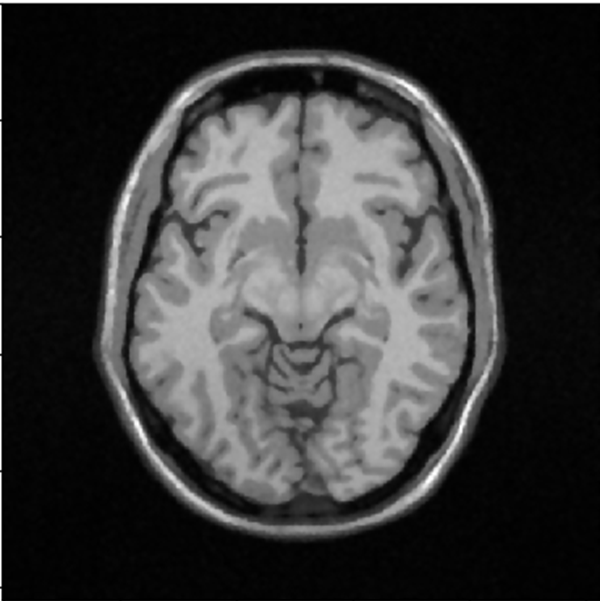
\includegraphics[scale=0.65]{figures/vis1}

\caption[Threads scheme]{\label{Fig:vis1}An example of the picture data for module 9. - Upsampling.}
\end{figure}


\begin{figure}
\centering
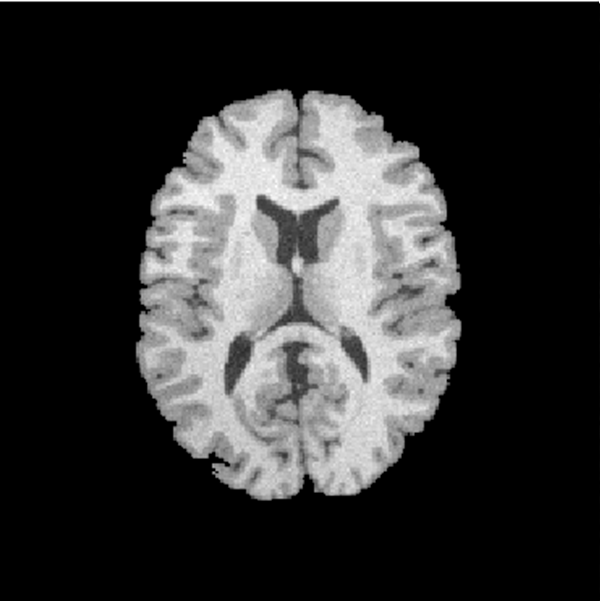
\includegraphics[scale=0.65]{figures/vis2}

\caption[Threads scheme]{\label{Fig:vis2}An example of the picture data for module 8. - Skull stripping.}
\end{figure}


The situation with the imaging of a 3D view on a 2D map is somewhat different. In this case, the matplotlib library was also used, but it was based on the "squezze" function, through which the color map, which represented the 3D image, was shown via the "FA" vector. A legend describing the observed picture was made for such a constituted image.


\begin{figure}
\centering
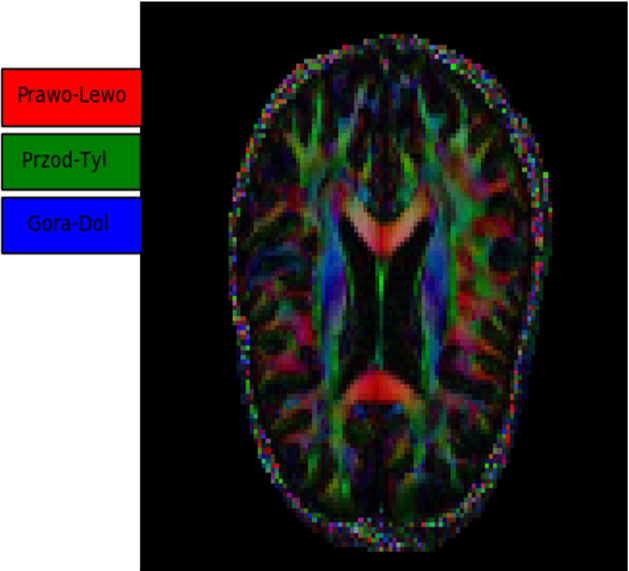
\includegraphics[scale=0.7]{figures/vis3}

\caption[Threads scheme]{\label{Fig:vis3}An example of the 3D RGB picture data for module 6. - Diffusion Tensor Imaging.}
\end{figure}


Results of the applied algorithm are shown on figure \ref{Fig:vis3}. 

An extremely important aspect of the application was the attachment of created images by following algorithms to the existing GUI. For this purpose, the "visualize" class was created, through which images were created in the QT window.

Below is an example code:

\begin{lstlisting}[language=Python, caption = Visualisation code connected with QT.]

import sys
from PyQt5.QtWidgets import QDialog, QApplication, QPushButton, QVBoxLayout
from matplotlib.backends.backend_qt5agg import FigureCanvasQTAgg as FigureCanvas
from matplotlib.backends.backend_qt5agg import NavigationToolbar2QT as NavigationToolbar
import matplotlib.pyplot as plt
import scipy.io

class Window(QDialog):
    def __init__(self, data):
        super(Window, self).__init__()
        self.data = data
        self.figure = plt.figure()
        self.canvas = FigureCanvas(self.figure)
        self.toolbar = NavigationToolbar(self.canvas, self)


        # set the layout
        layout = QVBoxLayout()
        layout.addWidget(self.toolbar)
        layout.addWidget(self.canvas)
        self.setLayout(layout)
        self.plot()

    def plot(self):
        ''' plot some random stuff '''
        mat = scipy.io.loadmat('recon_T1_synthetic_multiple_sclerosis_lesions_1mm_L16_r2.mat')
        self.axes = self.figure.add_subplot(111)               
        self.im1 = self.axes.imshow(self.data,cmap='hot', interpolation='nearest') 
        self.axes.axis('off')
        self.canvas.draw()

if __name__ == '__main__':
    mat = scipy.io.loadmat('recon_T1_synthetic_multiple_sclerosis_lesions_1mm_L16_r2.mat')
    data = mat['SENSE_LSE']

    app = QApplication(sys.argv)
    main = Window(data)
    main.show()
    sys.exit(app.exec_())

\end{lstlisting}

The result of the operation of connecting the visualized objects to the GUI is depicted on figure \ref{Fig:vis4}.



\begin{figure}
\centering
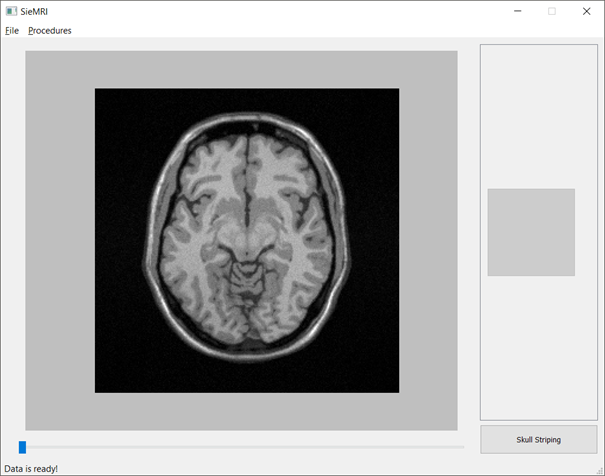
\includegraphics[scale=0.7]{figures/vis4}

\caption[Threads scheme]{\label{Fig:vis4}The illustrated data displayed in the GUI window.}
\end{figure}